% Options for packages loaded elsewhere
\PassOptionsToPackage{unicode}{hyperref}
\PassOptionsToPackage{hyphens}{url}
\PassOptionsToPackage{dvipsnames,svgnames,x11names}{xcolor}
%
\documentclass[
  letterpaper,
  DIV=11,
  numbers=noendperiod]{scrartcl}

\usepackage{amsmath,amssymb}
\usepackage{iftex}
\ifPDFTeX
  \usepackage[T1]{fontenc}
  \usepackage[utf8]{inputenc}
  \usepackage{textcomp} % provide euro and other symbols
\else % if luatex or xetex
  \usepackage{unicode-math}
  \defaultfontfeatures{Scale=MatchLowercase}
  \defaultfontfeatures[\rmfamily]{Ligatures=TeX,Scale=1}
\fi
\usepackage{lmodern}
\ifPDFTeX\else  
    % xetex/luatex font selection
\fi
% Use upquote if available, for straight quotes in verbatim environments
\IfFileExists{upquote.sty}{\usepackage{upquote}}{}
\IfFileExists{microtype.sty}{% use microtype if available
  \usepackage[]{microtype}
  \UseMicrotypeSet[protrusion]{basicmath} % disable protrusion for tt fonts
}{}
\makeatletter
\@ifundefined{KOMAClassName}{% if non-KOMA class
  \IfFileExists{parskip.sty}{%
    \usepackage{parskip}
  }{% else
    \setlength{\parindent}{0pt}
    \setlength{\parskip}{6pt plus 2pt minus 1pt}}
}{% if KOMA class
  \KOMAoptions{parskip=half}}
\makeatother
\usepackage{xcolor}
\setlength{\emergencystretch}{3em} % prevent overfull lines
\setcounter{secnumdepth}{-\maxdimen} % remove section numbering
% Make \paragraph and \subparagraph free-standing
\makeatletter
\ifx\paragraph\undefined\else
  \let\oldparagraph\paragraph
  \renewcommand{\paragraph}{
    \@ifstar
      \xxxParagraphStar
      \xxxParagraphNoStar
  }
  \newcommand{\xxxParagraphStar}[1]{\oldparagraph*{#1}\mbox{}}
  \newcommand{\xxxParagraphNoStar}[1]{\oldparagraph{#1}\mbox{}}
\fi
\ifx\subparagraph\undefined\else
  \let\oldsubparagraph\subparagraph
  \renewcommand{\subparagraph}{
    \@ifstar
      \xxxSubParagraphStar
      \xxxSubParagraphNoStar
  }
  \newcommand{\xxxSubParagraphStar}[1]{\oldsubparagraph*{#1}\mbox{}}
  \newcommand{\xxxSubParagraphNoStar}[1]{\oldsubparagraph{#1}\mbox{}}
\fi
\makeatother

\usepackage{color}
\usepackage{fancyvrb}
\newcommand{\VerbBar}{|}
\newcommand{\VERB}{\Verb[commandchars=\\\{\}]}
\DefineVerbatimEnvironment{Highlighting}{Verbatim}{commandchars=\\\{\}}
% Add ',fontsize=\small' for more characters per line
\usepackage{framed}
\definecolor{shadecolor}{RGB}{241,243,245}
\newenvironment{Shaded}{\begin{snugshade}}{\end{snugshade}}
\newcommand{\AlertTok}[1]{\textcolor[rgb]{0.68,0.00,0.00}{#1}}
\newcommand{\AnnotationTok}[1]{\textcolor[rgb]{0.37,0.37,0.37}{#1}}
\newcommand{\AttributeTok}[1]{\textcolor[rgb]{0.40,0.45,0.13}{#1}}
\newcommand{\BaseNTok}[1]{\textcolor[rgb]{0.68,0.00,0.00}{#1}}
\newcommand{\BuiltInTok}[1]{\textcolor[rgb]{0.00,0.23,0.31}{#1}}
\newcommand{\CharTok}[1]{\textcolor[rgb]{0.13,0.47,0.30}{#1}}
\newcommand{\CommentTok}[1]{\textcolor[rgb]{0.37,0.37,0.37}{#1}}
\newcommand{\CommentVarTok}[1]{\textcolor[rgb]{0.37,0.37,0.37}{\textit{#1}}}
\newcommand{\ConstantTok}[1]{\textcolor[rgb]{0.56,0.35,0.01}{#1}}
\newcommand{\ControlFlowTok}[1]{\textcolor[rgb]{0.00,0.23,0.31}{\textbf{#1}}}
\newcommand{\DataTypeTok}[1]{\textcolor[rgb]{0.68,0.00,0.00}{#1}}
\newcommand{\DecValTok}[1]{\textcolor[rgb]{0.68,0.00,0.00}{#1}}
\newcommand{\DocumentationTok}[1]{\textcolor[rgb]{0.37,0.37,0.37}{\textit{#1}}}
\newcommand{\ErrorTok}[1]{\textcolor[rgb]{0.68,0.00,0.00}{#1}}
\newcommand{\ExtensionTok}[1]{\textcolor[rgb]{0.00,0.23,0.31}{#1}}
\newcommand{\FloatTok}[1]{\textcolor[rgb]{0.68,0.00,0.00}{#1}}
\newcommand{\FunctionTok}[1]{\textcolor[rgb]{0.28,0.35,0.67}{#1}}
\newcommand{\ImportTok}[1]{\textcolor[rgb]{0.00,0.46,0.62}{#1}}
\newcommand{\InformationTok}[1]{\textcolor[rgb]{0.37,0.37,0.37}{#1}}
\newcommand{\KeywordTok}[1]{\textcolor[rgb]{0.00,0.23,0.31}{\textbf{#1}}}
\newcommand{\NormalTok}[1]{\textcolor[rgb]{0.00,0.23,0.31}{#1}}
\newcommand{\OperatorTok}[1]{\textcolor[rgb]{0.37,0.37,0.37}{#1}}
\newcommand{\OtherTok}[1]{\textcolor[rgb]{0.00,0.23,0.31}{#1}}
\newcommand{\PreprocessorTok}[1]{\textcolor[rgb]{0.68,0.00,0.00}{#1}}
\newcommand{\RegionMarkerTok}[1]{\textcolor[rgb]{0.00,0.23,0.31}{#1}}
\newcommand{\SpecialCharTok}[1]{\textcolor[rgb]{0.37,0.37,0.37}{#1}}
\newcommand{\SpecialStringTok}[1]{\textcolor[rgb]{0.13,0.47,0.30}{#1}}
\newcommand{\StringTok}[1]{\textcolor[rgb]{0.13,0.47,0.30}{#1}}
\newcommand{\VariableTok}[1]{\textcolor[rgb]{0.07,0.07,0.07}{#1}}
\newcommand{\VerbatimStringTok}[1]{\textcolor[rgb]{0.13,0.47,0.30}{#1}}
\newcommand{\WarningTok}[1]{\textcolor[rgb]{0.37,0.37,0.37}{\textit{#1}}}

\providecommand{\tightlist}{%
  \setlength{\itemsep}{0pt}\setlength{\parskip}{0pt}}\usepackage{longtable,booktabs,array}
\usepackage{calc} % for calculating minipage widths
% Correct order of tables after \paragraph or \subparagraph
\usepackage{etoolbox}
\makeatletter
\patchcmd\longtable{\par}{\if@noskipsec\mbox{}\fi\par}{}{}
\makeatother
% Allow footnotes in longtable head/foot
\IfFileExists{footnotehyper.sty}{\usepackage{footnotehyper}}{\usepackage{footnote}}
\makesavenoteenv{longtable}
\usepackage{graphicx}
\makeatletter
\def\maxwidth{\ifdim\Gin@nat@width>\linewidth\linewidth\else\Gin@nat@width\fi}
\def\maxheight{\ifdim\Gin@nat@height>\textheight\textheight\else\Gin@nat@height\fi}
\makeatother
% Scale images if necessary, so that they will not overflow the page
% margins by default, and it is still possible to overwrite the defaults
% using explicit options in \includegraphics[width, height, ...]{}
\setkeys{Gin}{width=\maxwidth,height=\maxheight,keepaspectratio}
% Set default figure placement to htbp
\makeatletter
\def\fps@figure{htbp}
\makeatother

\usepackage{fvextra}
\DefineVerbatimEnvironment{Highlighting}{Verbatim}{breaklines,commandchars=\\\{\}}
\KOMAoption{captions}{tableheading}
\makeatletter
\@ifpackageloaded{caption}{}{\usepackage{caption}}
\AtBeginDocument{%
\ifdefined\contentsname
  \renewcommand*\contentsname{Table of contents}
\else
  \newcommand\contentsname{Table of contents}
\fi
\ifdefined\listfigurename
  \renewcommand*\listfigurename{List of Figures}
\else
  \newcommand\listfigurename{List of Figures}
\fi
\ifdefined\listtablename
  \renewcommand*\listtablename{List of Tables}
\else
  \newcommand\listtablename{List of Tables}
\fi
\ifdefined\figurename
  \renewcommand*\figurename{Figure}
\else
  \newcommand\figurename{Figure}
\fi
\ifdefined\tablename
  \renewcommand*\tablename{Table}
\else
  \newcommand\tablename{Table}
\fi
}
\@ifpackageloaded{float}{}{\usepackage{float}}
\floatstyle{ruled}
\@ifundefined{c@chapter}{\newfloat{codelisting}{h}{lop}}{\newfloat{codelisting}{h}{lop}[chapter]}
\floatname{codelisting}{Listing}
\newcommand*\listoflistings{\listof{codelisting}{List of Listings}}
\makeatother
\makeatletter
\makeatother
\makeatletter
\@ifpackageloaded{caption}{}{\usepackage{caption}}
\@ifpackageloaded{subcaption}{}{\usepackage{subcaption}}
\makeatother

\ifLuaTeX
  \usepackage{selnolig}  % disable illegal ligatures
\fi
\usepackage{bookmark}

\IfFileExists{xurl.sty}{\usepackage{xurl}}{} % add URL line breaks if available
\urlstyle{same} % disable monospaced font for URLs
\hypersetup{
  pdftitle={ML-PS4},
  pdfauthor={Duoshu Xu},
  colorlinks=true,
  linkcolor={blue},
  filecolor={Maroon},
  citecolor={Blue},
  urlcolor={Blue},
  pdfcreator={LaTeX via pandoc}}


\title{ML-PS4}
\author{Duoshu Xu}
\date{}

\begin{document}
\maketitle

\RecustomVerbatimEnvironment{verbatim}{Verbatim}{
  showspaces = false,
  showtabs = false,
  breaksymbolleft={},
  breaklines
}


\textbf{Partnered with Jae Hu}

\begin{Shaded}
\begin{Highlighting}[]
\ImportTok{import}\NormalTok{ pandas }\ImportTok{as}\NormalTok{ pd}
\ImportTok{import}\NormalTok{ numpy }\ImportTok{as}\NormalTok{ np}
\ImportTok{from}\NormalTok{ sklearn.model\_selection }\ImportTok{import}\NormalTok{ train\_test\_split}
\ImportTok{from}\NormalTok{ sklearn.preprocessing }\ImportTok{import}\NormalTok{ StandardScaler}
\ImportTok{from}\NormalTok{ sklearn.linear\_model }\ImportTok{import}\NormalTok{ LinearRegression}
\ImportTok{from}\NormalTok{ sklearn.metrics }\ImportTok{import}\NormalTok{ mean\_squared\_error}
\ImportTok{from}\NormalTok{ sklearn.decomposition }\ImportTok{import}\NormalTok{ PCA}
\ImportTok{from}\NormalTok{ sklearn.model\_selection }\ImportTok{import}\NormalTok{ cross\_val\_score, KFold}
\ImportTok{from}\NormalTok{ sklearn.cross\_decomposition }\ImportTok{import}\NormalTok{ PLSRegression}
\ImportTok{import}\NormalTok{ networkx }\ImportTok{as}\NormalTok{ nx}
\ImportTok{import}\NormalTok{ matplotlib.pyplot }\ImportTok{as}\NormalTok{ plt}
\ImportTok{from}\NormalTok{ sklearn.tree }\ImportTok{import}\NormalTok{ DecisionTreeClassifier}
\ImportTok{from}\NormalTok{ sklearn.metrics }\ImportTok{import}\NormalTok{ accuracy\_score}
\ImportTok{from}\NormalTok{ sklearn.preprocessing }\ImportTok{import}\NormalTok{ LabelEncoder}
\ImportTok{from}\NormalTok{ sklearn.tree }\ImportTok{import}\NormalTok{ plot\_tree}
\ImportTok{from}\NormalTok{ sklearn.metrics }\ImportTok{import}\NormalTok{ confusion\_matrix}
\end{Highlighting}
\end{Shaded}

\section{Question 1}\label{question-1}

\begin{Shaded}
\begin{Highlighting}[]
\CommentTok{\# load the dataset}
\NormalTok{file\_path }\OperatorTok{=} \StringTok{"/Users/kevinxu/Documents/GitHub/ML{-}PS4/Data{-}College.csv"}
\NormalTok{college\_df }\OperatorTok{=}\NormalTok{ pd.read\_csv(file\_path)}
\end{Highlighting}
\end{Shaded}

\subsection{Question 1a}\label{question-1a}

\begin{Shaded}
\begin{Highlighting}[]
\CommentTok{\# drop the first column which is the name of the university}
\NormalTok{college\_df }\OperatorTok{=}\NormalTok{ college\_df.drop(columns}\OperatorTok{=}\NormalTok{[}\StringTok{\textquotesingle{}Unnamed: 0\textquotesingle{}}\NormalTok{])}

\CommentTok{\# convert categorical column \textquotesingle{}Private\textquotesingle{} to numerical}
\NormalTok{college\_df[}\StringTok{\textquotesingle{}Private\textquotesingle{}}\NormalTok{] }\OperatorTok{=}\NormalTok{ college\_df[}\StringTok{\textquotesingle{}Private\textquotesingle{}}\NormalTok{].}\BuiltInTok{map}\NormalTok{(\{}\StringTok{\textquotesingle{}Yes\textquotesingle{}}\NormalTok{: }\DecValTok{1}\NormalTok{, }\StringTok{\textquotesingle{}No\textquotesingle{}}\NormalTok{: }\DecValTok{0}\NormalTok{\})}

\CommentTok{\# define predictors and target variable}
\NormalTok{X }\OperatorTok{=}\NormalTok{ college\_df.drop(columns}\OperatorTok{=}\NormalTok{[}\StringTok{\textquotesingle{}Apps\textquotesingle{}}\NormalTok{])}
\NormalTok{y }\OperatorTok{=}\NormalTok{ college\_df[}\StringTok{\textquotesingle{}Apps\textquotesingle{}}\NormalTok{]}

\CommentTok{\# split the data into training and testing sets}
\NormalTok{X\_train, X\_test, y\_train, y\_test }\OperatorTok{=}\NormalTok{ train\_test\_split(}
\NormalTok{    X, y, test\_size}\OperatorTok{=}\FloatTok{0.5}\NormalTok{, random\_state}\OperatorTok{=}\DecValTok{37}\NormalTok{)}

\CommentTok{\# scale the predictors}
\NormalTok{scaler }\OperatorTok{=}\NormalTok{ StandardScaler()}
\NormalTok{X\_train\_scaled }\OperatorTok{=}\NormalTok{ scaler.fit\_transform(X\_train)}
\NormalTok{X\_test\_scaled }\OperatorTok{=}\NormalTok{ scaler.transform(X\_test)}

\CommentTok{\# convert scaled data back to DataFrame}
\NormalTok{X\_train\_scaled\_college\_df }\OperatorTok{=}\NormalTok{ pd.DataFrame(X\_train\_scaled, columns}\OperatorTok{=}\NormalTok{X.columns)}
\NormalTok{X\_test\_scaled\_college\_df }\OperatorTok{=}\NormalTok{ pd.DataFrame(X\_test\_scaled, columns}\OperatorTok{=}\NormalTok{X.columns)}
\end{Highlighting}
\end{Shaded}

\subsection{Question 1b}\label{question-1b}

\begin{Shaded}
\begin{Highlighting}[]
\CommentTok{\# fit a linear regression model}
\NormalTok{lm }\OperatorTok{=}\NormalTok{ LinearRegression()}
\NormalTok{lm.fit(X\_train\_scaled, y\_train)}

\CommentTok{\# predict on the test set}
\NormalTok{y\_pred }\OperatorTok{=}\NormalTok{ lm.predict(X\_test\_scaled)}
\NormalTok{test\_mse }\OperatorTok{=}\NormalTok{ mean\_squared\_error(y\_test, y\_pred)}
\NormalTok{test\_mse}
\end{Highlighting}
\end{Shaded}

\begin{verbatim}
1222954.0382534422
\end{verbatim}

\begin{itemize}
\tightlist
\item
  Test MSE: 1222954.0382534422
\end{itemize}

\subsection{Question 1c}\label{question-1c}

\begin{Shaded}
\begin{Highlighting}[]
\CommentTok{\# define 10{-}fold cross{-}validation}
\NormalTok{kf }\OperatorTok{=}\NormalTok{ KFold(n\_splits}\OperatorTok{=}\DecValTok{10}\NormalTok{, shuffle}\OperatorTok{=}\VariableTok{True}\NormalTok{, random\_state}\OperatorTok{=}\DecValTok{1}\NormalTok{)}

\CommentTok{\# perform PCA on training data}
\NormalTok{pca }\OperatorTok{=}\NormalTok{ PCA()}
\NormalTok{X\_train\_pca }\OperatorTok{=}\NormalTok{ pca.fit\_transform(X\_train\_scaled)}
\NormalTok{X\_test\_pca }\OperatorTok{=}\NormalTok{ pca.transform(X\_test\_scaled)}

\CommentTok{\# find the optimal number of principal components}
\NormalTok{mse\_list }\OperatorTok{=}\NormalTok{ []}
\NormalTok{components\_range }\OperatorTok{=} \BuiltInTok{range}\NormalTok{(}\DecValTok{1}\NormalTok{, X\_train\_scaled.shape[}\DecValTok{1}\NormalTok{] }\OperatorTok{+} \DecValTok{1}\NormalTok{)}

\ControlFlowTok{for}\NormalTok{ m }\KeywordTok{in}\NormalTok{ components\_range:}
\NormalTok{    X\_train\_pca\_m }\OperatorTok{=}\NormalTok{ X\_train\_pca[:, :m]}
\NormalTok{    lm\_pcr }\OperatorTok{=}\NormalTok{ LinearRegression()}
\NormalTok{    mse }\OperatorTok{=} \OperatorTok{{-}}\NormalTok{np.mean(cross\_val\_score(lm\_pcr, X\_train\_pca\_m,}
\NormalTok{                   y\_train, cv}\OperatorTok{=}\NormalTok{kf, scoring}\OperatorTok{=}\StringTok{\textquotesingle{}neg\_mean\_squared\_error\textquotesingle{}}\NormalTok{))}
\NormalTok{    mse\_list.append(mse)}

\NormalTok{optimal\_m }\OperatorTok{=}\NormalTok{ components\_range[np.argmin(mse\_list)]}

\CommentTok{\# fit PCR model using optimal number of components}
\NormalTok{X\_train\_pca\_opt }\OperatorTok{=}\NormalTok{ X\_train\_pca[:, :optimal\_m]}
\NormalTok{X\_test\_pca\_opt }\OperatorTok{=}\NormalTok{ X\_test\_pca[:, :optimal\_m]}
\NormalTok{lm\_pcr\_opt }\OperatorTok{=}\NormalTok{ LinearRegression()}
\NormalTok{lm\_pcr\_opt.fit(X\_train\_pca\_opt, y\_train)}
\NormalTok{y\_pcr\_pred }\OperatorTok{=}\NormalTok{ lm\_pcr\_opt.predict(X\_test\_pca\_opt)}

\CommentTok{\# compute MSE}
\NormalTok{test\_mse\_pcr }\OperatorTok{=}\NormalTok{ mean\_squared\_error(y\_test, y\_pcr\_pred)}

\CommentTok{\# determine the elbow point using the "elbow method"}
\NormalTok{second\_derivative }\OperatorTok{=}\NormalTok{ np.diff(mse\_list, }\DecValTok{2}\NormalTok{)}
\NormalTok{elbow\_m }\OperatorTok{=}\NormalTok{ components\_range[np.argmin(second\_derivative) }\OperatorTok{+} \DecValTok{1}\NormalTok{]}

\NormalTok{optimal\_m, test\_mse\_pcr, elbow\_m}
\end{Highlighting}
\end{Shaded}

\begin{verbatim}
(16, 1487304.1279126806, 3)
\end{verbatim}

\subsection{Question 1d}\label{question-1d}

\begin{Shaded}
\begin{Highlighting}[]
\CommentTok{\# select the optimal number of components for PLS}
\NormalTok{mse\_list\_pls }\OperatorTok{=}\NormalTok{ []}

\ControlFlowTok{for}\NormalTok{ m }\KeywordTok{in}\NormalTok{ components\_range:}
\NormalTok{    pls }\OperatorTok{=}\NormalTok{ PLSRegression(n\_components}\OperatorTok{=}\NormalTok{m)}
\NormalTok{    mse }\OperatorTok{=} \OperatorTok{{-}}\NormalTok{np.mean(cross\_val\_score(pls, X\_train\_scaled, y\_train,}
\NormalTok{                   cv}\OperatorTok{=}\NormalTok{kf, scoring}\OperatorTok{=}\StringTok{\textquotesingle{}neg\_mean\_squared\_error\textquotesingle{}}\NormalTok{))}
\NormalTok{    mse\_list\_pls.append(mse)}

\CommentTok{\# minimizing cross{-}validated error}
\NormalTok{optimal\_m\_pls }\OperatorTok{=}\NormalTok{ components\_range[np.argmin(mse\_list\_pls)]}

\CommentTok{\# fit PLS model}
\NormalTok{pls\_opt }\OperatorTok{=}\NormalTok{ PLSRegression(n\_components}\OperatorTok{=}\NormalTok{optimal\_m\_pls)}
\NormalTok{pls\_opt.fit(X\_train\_scaled, y\_train)}
\NormalTok{y\_pls\_pred }\OperatorTok{=}\NormalTok{ pls\_opt.predict(X\_test\_scaled)}

\CommentTok{\# compute MSE}
\NormalTok{test\_mse\_pls }\OperatorTok{=}\NormalTok{ mean\_squared\_error(y\_test, y\_pls\_pred)}

\CommentTok{\# determine the elbow point}
\NormalTok{second\_derivative\_pls }\OperatorTok{=}\NormalTok{ np.diff(mse\_list\_pls, }\DecValTok{2}\NormalTok{)}
\NormalTok{elbow\_m\_pls }\OperatorTok{=}\NormalTok{ components\_range[np.argmin(second\_derivative\_pls) }\OperatorTok{+} \DecValTok{1}\NormalTok{]}

\NormalTok{optimal\_m\_pls, test\_mse\_pls, elbow\_m\_pls}
\end{Highlighting}
\end{Shaded}

\begin{verbatim}
(9, 1300987.697197346, 4)
\end{verbatim}

\subsection{Question 1e}\label{question-1e}

\begin{itemize}
\tightlist
\item
  The linear regression model (OLS) performed best with the lowest test
  error (1,222,954.04), indicating that all predictors provided valuable
  information and there was no significant multicollinearity problem.
  The PLS model (1,300,987.70) performed better than the PCR
  (1,487,304.13) because it took into account the information of the
  response variable during the dimensionality reduction process. Both
  the PCR and PLS models showed high errors, suggesting that the
  dimensionality reduction process may have lost some important
  predictive information. Overall, the OLS model remained the most
  effective prediction tool, while the PLS model provided a good balance
  between model complexity and prediction performance.
\end{itemize}

\section{Question 2}\label{question-2}

\subsection{Question 2a}\label{question-2a}

\begin{Shaded}
\begin{Highlighting}[]
\CommentTok{\# reate a decision tree graph}
\NormalTok{G }\OperatorTok{=}\NormalTok{ nx.DiGraph()}

\CommentTok{\# adding nodes}
\NormalTok{G.add\_node(}\StringTok{"Root"}\NormalTok{)}
\NormalTok{G.add\_node(}\StringTok{"X2 \textless{} 1"}\NormalTok{)}
\NormalTok{G.add\_node(}\StringTok{"X1 \textless{} 1"}\NormalTok{)}
\NormalTok{G.add\_node(}\StringTok{"X1 \textless{} 0"}\NormalTok{)}
\NormalTok{G.add\_node(}\StringTok{"X2 \textless{} 0"}\NormalTok{)}
\NormalTok{G.add\_node(}\StringTok{"3"}\NormalTok{)}
\NormalTok{G.add\_node(}\StringTok{"10"}\NormalTok{)}
\NormalTok{G.add\_node(}\StringTok{"0"}\NormalTok{)}
\NormalTok{G.add\_node(}\StringTok{"15"}\NormalTok{)}
\NormalTok{G.add\_node(}\StringTok{"5"}\NormalTok{)}

\CommentTok{\# adding edges}
\NormalTok{G.add\_edges\_from([}
\NormalTok{    (}\StringTok{"Root"}\NormalTok{, }\StringTok{"X2 \textless{} 1"}\NormalTok{), (}\StringTok{"X2 \textless{} 1"}\NormalTok{, }\StringTok{"X1 \textless{} 1"}\NormalTok{), (}\StringTok{"X1 \textless{} 1"}\NormalTok{,}
                                               \StringTok{"X1 \textless{} 0"}\NormalTok{), (}\StringTok{"X1 \textless{} 0"}\NormalTok{, }\StringTok{"3"}\NormalTok{), (}\StringTok{"X1 \textless{} 0"}\NormalTok{, }\StringTok{"X2 \textless{} 0"}\NormalTok{),}
\NormalTok{    (}\StringTok{"X2 \textless{} 0"}\NormalTok{, }\StringTok{"10"}\NormalTok{), (}\StringTok{"X2 \textless{} 0"}\NormalTok{, }\StringTok{"0"}\NormalTok{), (}\StringTok{"X1 \textless{} 1"}\NormalTok{, }\StringTok{"15"}\NormalTok{), (}\StringTok{"X2 \textless{} 1"}\NormalTok{, }\StringTok{"5"}\NormalTok{)}
\NormalTok{])}

\CommentTok{\# define positions}
\NormalTok{pos }\OperatorTok{=}\NormalTok{ \{}
    \StringTok{"Root"}\NormalTok{: (}\DecValTok{2}\NormalTok{, }\DecValTok{4}\NormalTok{),}
    \StringTok{"X2 \textless{} 1"}\NormalTok{: (}\DecValTok{2}\NormalTok{, }\DecValTok{3}\NormalTok{),}
    \StringTok{"X1 \textless{} 1"}\NormalTok{: (}\DecValTok{1}\NormalTok{, }\DecValTok{2}\NormalTok{),}
    \StringTok{"X1 \textless{} 0"}\NormalTok{: (}\DecValTok{0}\NormalTok{, }\DecValTok{1}\NormalTok{),}
    \StringTok{"X2 \textless{} 0"}\NormalTok{: (}\DecValTok{1}\NormalTok{, }\DecValTok{1}\NormalTok{),}
    \StringTok{"3"}\NormalTok{: (}\OperatorTok{{-}}\DecValTok{1}\NormalTok{, }\DecValTok{0}\NormalTok{),}
    \StringTok{"10"}\NormalTok{: (}\DecValTok{0}\NormalTok{, }\DecValTok{0}\NormalTok{),}
    \StringTok{"0"}\NormalTok{: (}\DecValTok{2}\NormalTok{, }\DecValTok{0}\NormalTok{),}
    \StringTok{"15"}\NormalTok{: (}\DecValTok{3}\NormalTok{, }\DecValTok{2}\NormalTok{),}
    \StringTok{"5"}\NormalTok{: (}\DecValTok{4}\NormalTok{, }\DecValTok{3}\NormalTok{)}
\NormalTok{\}}

\CommentTok{\# display the graph}
\NormalTok{plt.figure(figsize}\OperatorTok{=}\NormalTok{(}\DecValTok{8}\NormalTok{, }\DecValTok{6}\NormalTok{))}
\NormalTok{nx.draw(G, pos, with\_labels}\OperatorTok{=}\VariableTok{True}\NormalTok{, node\_size}\OperatorTok{=}\DecValTok{3000}\NormalTok{, node\_color}\OperatorTok{=}\StringTok{"lightblue"}\NormalTok{,}
\NormalTok{        font\_size}\OperatorTok{=}\DecValTok{10}\NormalTok{, font\_weight}\OperatorTok{=}\StringTok{"bold"}\NormalTok{, edge\_color}\OperatorTok{=}\StringTok{"gray"}\NormalTok{)}
\NormalTok{plt.title(}\StringTok{"Decision Tree"}\NormalTok{)}
\NormalTok{plt.show()}
\end{Highlighting}
\end{Shaded}

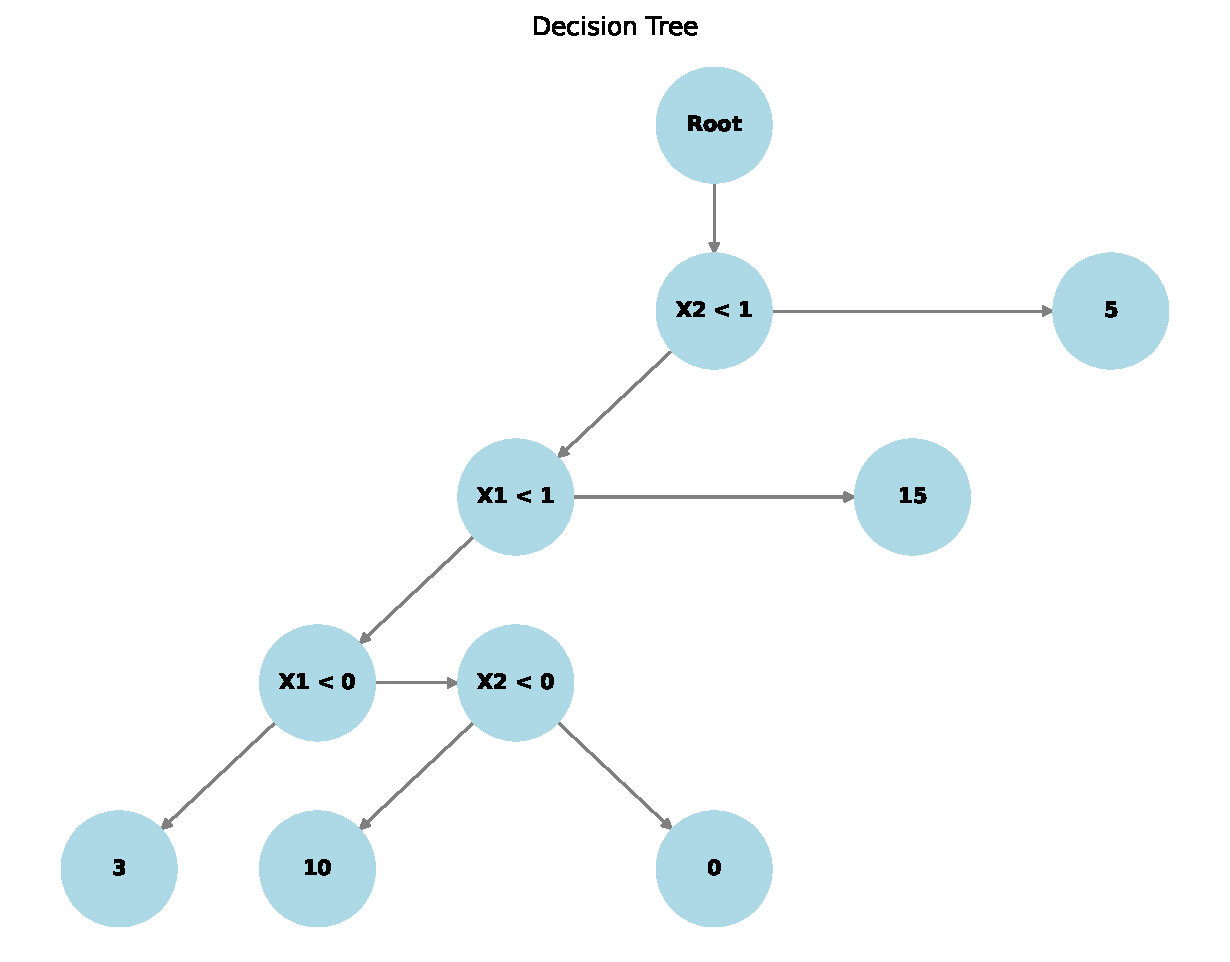
\includegraphics{PS4_files/figure-pdf/cell-8-output-1.pdf}

\subsection{Question 2b}\label{question-2b}

\begin{Shaded}
\begin{Highlighting}[]
\NormalTok{fig, ax }\OperatorTok{=}\NormalTok{ plt.subplots(figsize}\OperatorTok{=}\NormalTok{(}\DecValTok{6}\NormalTok{, }\DecValTok{6}\NormalTok{))}

\CommentTok{\# set limits and labels}
\NormalTok{ax.set\_xlim(}\OperatorTok{{-}}\DecValTok{1}\NormalTok{, }\DecValTok{2}\NormalTok{)}
\NormalTok{ax.set\_ylim(}\DecValTok{0}\NormalTok{, }\DecValTok{3}\NormalTok{)}
\NormalTok{ax.set\_xlabel(}\StringTok{"X1"}\NormalTok{)}
\NormalTok{ax.set\_ylabel(}\StringTok{"X2"}\NormalTok{)}

\CommentTok{\# draw partition lines}
\NormalTok{ax.axhline(y}\OperatorTok{=}\DecValTok{1}\NormalTok{, color}\OperatorTok{=}\StringTok{"red"}\NormalTok{, linestyle}\OperatorTok{=}\StringTok{"dashed"}\NormalTok{)}
\NormalTok{ax.axhline(y}\OperatorTok{=}\DecValTok{2}\NormalTok{, color}\OperatorTok{=}\StringTok{"red"}\NormalTok{, linestyle}\OperatorTok{=}\StringTok{"dashed"}\NormalTok{)}
\NormalTok{ax.vlines(x}\OperatorTok{=}\DecValTok{1}\NormalTok{, ymin}\OperatorTok{=}\DecValTok{0}\NormalTok{, ymax}\OperatorTok{=}\DecValTok{1}\NormalTok{, color}\OperatorTok{=}\StringTok{"blue"}\NormalTok{, linestyle}\OperatorTok{=}\StringTok{"dashed"}\NormalTok{)}
\NormalTok{ax.vlines(x}\OperatorTok{=}\DecValTok{0}\NormalTok{, ymin}\OperatorTok{=}\DecValTok{1}\NormalTok{, ymax}\OperatorTok{=}\DecValTok{2}\NormalTok{, color}\OperatorTok{=}\StringTok{"blue"}\NormalTok{, linestyle}\OperatorTok{=}\StringTok{"dashed"}\NormalTok{)}

\CommentTok{\# add region labels (mean values from the tree)}
\NormalTok{ax.text(}\DecValTok{0}\NormalTok{, }\FloatTok{0.5}\NormalTok{, }\StringTok{"{-}1.80"}\NormalTok{, fontsize}\OperatorTok{=}\DecValTok{12}\NormalTok{, ha}\OperatorTok{=}\StringTok{\textquotesingle{}center\textquotesingle{}}\NormalTok{, va}\OperatorTok{=}\StringTok{\textquotesingle{}center\textquotesingle{}}\NormalTok{)}
\NormalTok{ax.text(}\FloatTok{1.5}\NormalTok{, }\FloatTok{0.5}\NormalTok{, }\StringTok{"0.63"}\NormalTok{, fontsize}\OperatorTok{=}\DecValTok{12}\NormalTok{, ha}\OperatorTok{=}\StringTok{\textquotesingle{}center\textquotesingle{}}\NormalTok{, va}\OperatorTok{=}\StringTok{\textquotesingle{}center\textquotesingle{}}\NormalTok{)}
\NormalTok{ax.text(}\OperatorTok{{-}}\FloatTok{0.5}\NormalTok{, }\FloatTok{1.5}\NormalTok{, }\StringTok{"{-}1.06"}\NormalTok{, fontsize}\OperatorTok{=}\DecValTok{12}\NormalTok{, ha}\OperatorTok{=}\StringTok{\textquotesingle{}center\textquotesingle{}}\NormalTok{, va}\OperatorTok{=}\StringTok{\textquotesingle{}center\textquotesingle{}}\NormalTok{)}
\NormalTok{ax.text(}\DecValTok{1}\NormalTok{, }\FloatTok{1.5}\NormalTok{, }\StringTok{"0.21"}\NormalTok{, fontsize}\OperatorTok{=}\DecValTok{12}\NormalTok{, ha}\OperatorTok{=}\StringTok{\textquotesingle{}center\textquotesingle{}}\NormalTok{, va}\OperatorTok{=}\StringTok{\textquotesingle{}center\textquotesingle{}}\NormalTok{)}
\NormalTok{ax.text(}\FloatTok{0.5}\NormalTok{, }\FloatTok{2.5}\NormalTok{, }\StringTok{"2.49"}\NormalTok{, fontsize}\OperatorTok{=}\DecValTok{12}\NormalTok{, ha}\OperatorTok{=}\StringTok{\textquotesingle{}center\textquotesingle{}}\NormalTok{, va}\OperatorTok{=}\StringTok{\textquotesingle{}center\textquotesingle{}}\NormalTok{)}

\CommentTok{\# display the plot}
\NormalTok{plt.title(}\StringTok{"Partition Diagram"}\NormalTok{)}
\NormalTok{plt.show()}
\end{Highlighting}
\end{Shaded}

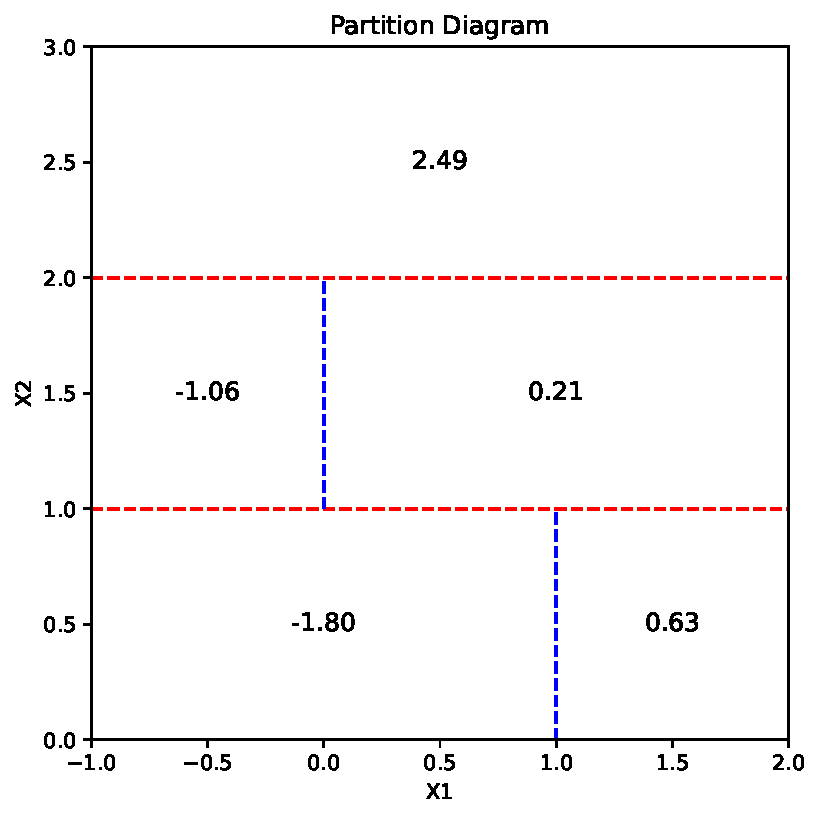
\includegraphics{PS4_files/figure-pdf/cell-9-output-1.pdf}

\section{Question 3}\label{question-3}

\begin{Shaded}
\begin{Highlighting}[]
\NormalTok{oj\_file\_path }\OperatorTok{=} \StringTok{"/Users/kevinxu/Documents/GitHub/ML{-}PS4/Data{-}OJ.csv"}
\NormalTok{oj\_df }\OperatorTok{=}\NormalTok{ pd.read\_csv(oj\_file\_path)}
\end{Highlighting}
\end{Shaded}

\subsection{Question 3a}\label{question-3a}

\begin{Shaded}
\begin{Highlighting}[]
\CommentTok{\# define variable}
\NormalTok{X }\OperatorTok{=}\NormalTok{ oj\_df.drop(columns}\OperatorTok{=}\NormalTok{[}\StringTok{\textquotesingle{}Purchase\textquotesingle{}}\NormalTok{])}
\NormalTok{y }\OperatorTok{=}\NormalTok{ oj\_df[}\StringTok{\textquotesingle{}Purchase\textquotesingle{}}\NormalTok{]}

\CommentTok{\# split the data into training and testing sets}
\NormalTok{X\_train, X\_test, y\_train, y\_test }\OperatorTok{=}\NormalTok{ train\_test\_split(}
\NormalTok{    X, y, test\_size}\OperatorTok{=}\FloatTok{0.3}\NormalTok{, random\_state}\OperatorTok{=}\DecValTok{3}\NormalTok{)}
\end{Highlighting}
\end{Shaded}

\subsection{Question 3b}\label{question-3b}

\begin{Shaded}
\begin{Highlighting}[]
\CommentTok{\# encode the target variable}
\NormalTok{y\_train\_encoded }\OperatorTok{=}\NormalTok{ LabelEncoder().fit\_transform(y\_train)}
\NormalTok{y\_test\_encoded }\OperatorTok{=}\NormalTok{ LabelEncoder().fit\_transform(y\_test)}

\CommentTok{\# convert categorical predictors to numeric values}
\NormalTok{X\_train\_encoded }\OperatorTok{=}\NormalTok{ pd.get\_dummies(X\_train, drop\_first}\OperatorTok{=}\VariableTok{True}\NormalTok{)}
\NormalTok{X\_test\_encoded }\OperatorTok{=}\NormalTok{ pd.get\_dummies(X\_test, drop\_first}\OperatorTok{=}\VariableTok{True}\NormalTok{)}

\NormalTok{X\_train\_encoded, X\_test\_encoded }\OperatorTok{=}\NormalTok{ X\_train\_encoded.align(}
\NormalTok{    X\_test\_encoded, join}\OperatorTok{=}\StringTok{\textquotesingle{}left\textquotesingle{}}\NormalTok{, axis}\OperatorTok{=}\DecValTok{1}\NormalTok{, fill\_value}\OperatorTok{=}\DecValTok{0}\NormalTok{)}

\CommentTok{\# fit the full decision tree model}
\NormalTok{tree\_clf }\OperatorTok{=}\NormalTok{ DecisionTreeClassifier(random\_state}\OperatorTok{=}\DecValTok{2}\NormalTok{)}
\NormalTok{tree\_clf.fit(X\_train\_encoded, y\_train\_encoded)}

\CommentTok{\# predict on the training set}
\NormalTok{y\_train\_pred }\OperatorTok{=}\NormalTok{ tree\_clf.predict(X\_train\_encoded)}

\CommentTok{\# compute and display the training error rate}
\NormalTok{train\_error\_rate }\OperatorTok{=} \DecValTok{1} \OperatorTok{{-}}\NormalTok{ accuracy\_score(y\_train\_encoded, y\_train\_pred)}
\NormalTok{train\_error\_rate}
\end{Highlighting}
\end{Shaded}

\begin{verbatim}
0.006675567423230944
\end{verbatim}

\subsection{Question 3c}\label{question-3c}

\begin{Shaded}
\begin{Highlighting}[]
\CommentTok{\# plot the full, unpruned tree}
\NormalTok{plt.figure(figsize}\OperatorTok{=}\NormalTok{(}\DecValTok{15}\NormalTok{, }\DecValTok{8}\NormalTok{))}
\NormalTok{plot\_tree(tree\_clf, feature\_names}\OperatorTok{=}\NormalTok{X\_train\_encoded.columns,}
\NormalTok{          class\_names}\OperatorTok{=}\NormalTok{[}\StringTok{\textquotesingle{}CH\textquotesingle{}}\NormalTok{, }\StringTok{\textquotesingle{}MM\textquotesingle{}}\NormalTok{], filled}\OperatorTok{=}\VariableTok{True}\NormalTok{, fontsize}\OperatorTok{=}\DecValTok{6}\NormalTok{)}
\NormalTok{plt.title(}\StringTok{"Full Unpruned Decision Tree"}\NormalTok{)}
\NormalTok{plt.show()}

\CommentTok{\# fit a pruned decision tree}
\NormalTok{tree\_clf\_pruned }\OperatorTok{=}\NormalTok{ DecisionTreeClassifier(max\_depth}\OperatorTok{=}\DecValTok{3}\NormalTok{, random\_state}\OperatorTok{=}\DecValTok{2}\NormalTok{)}
\NormalTok{tree\_clf\_pruned.fit(X\_train\_encoded, y\_train\_encoded)}

\CommentTok{\# plot the pruned tree}
\NormalTok{plt.figure(figsize}\OperatorTok{=}\NormalTok{(}\DecValTok{12}\NormalTok{, }\DecValTok{6}\NormalTok{))}
\NormalTok{plot\_tree(tree\_clf\_pruned, feature\_names}\OperatorTok{=}\NormalTok{X\_train\_encoded.columns,}
\NormalTok{          class\_names}\OperatorTok{=}\NormalTok{[}\StringTok{\textquotesingle{}CH\textquotesingle{}}\NormalTok{, }\StringTok{\textquotesingle{}MM\textquotesingle{}}\NormalTok{], filled}\OperatorTok{=}\VariableTok{True}\NormalTok{, fontsize}\OperatorTok{=}\DecValTok{10}\NormalTok{)}
\NormalTok{plt.title(}\StringTok{"Pruned Decision Tree (Max Depth = 3)"}\NormalTok{)}
\NormalTok{plt.show()}

\CommentTok{\# count the number of terminal nodes}
\NormalTok{num\_terminal\_nodes }\OperatorTok{=} \BuiltInTok{sum}\NormalTok{(tree\_clf\_pruned.tree\_.children\_left }\OperatorTok{==} \OperatorTok{{-}}\DecValTok{1}\NormalTok{)}

\NormalTok{num\_terminal\_nodes}
\end{Highlighting}
\end{Shaded}

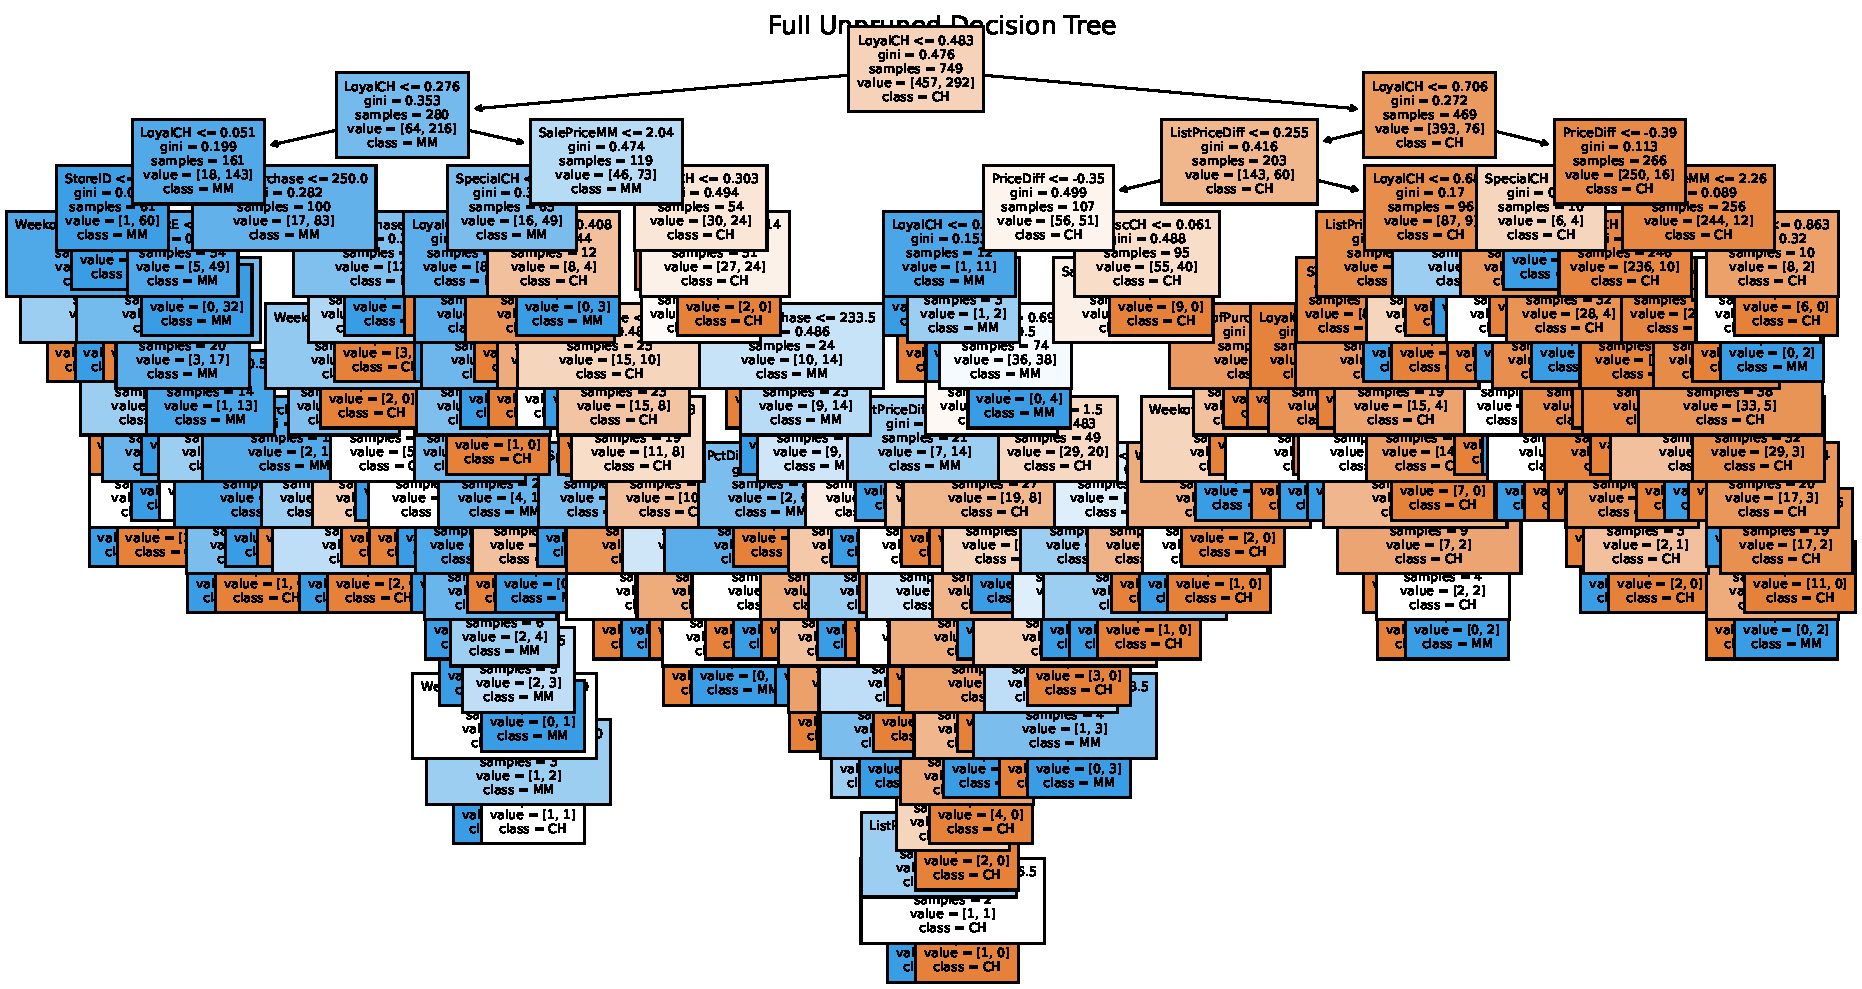
\includegraphics{PS4_files/figure-pdf/cell-13-output-1.pdf}

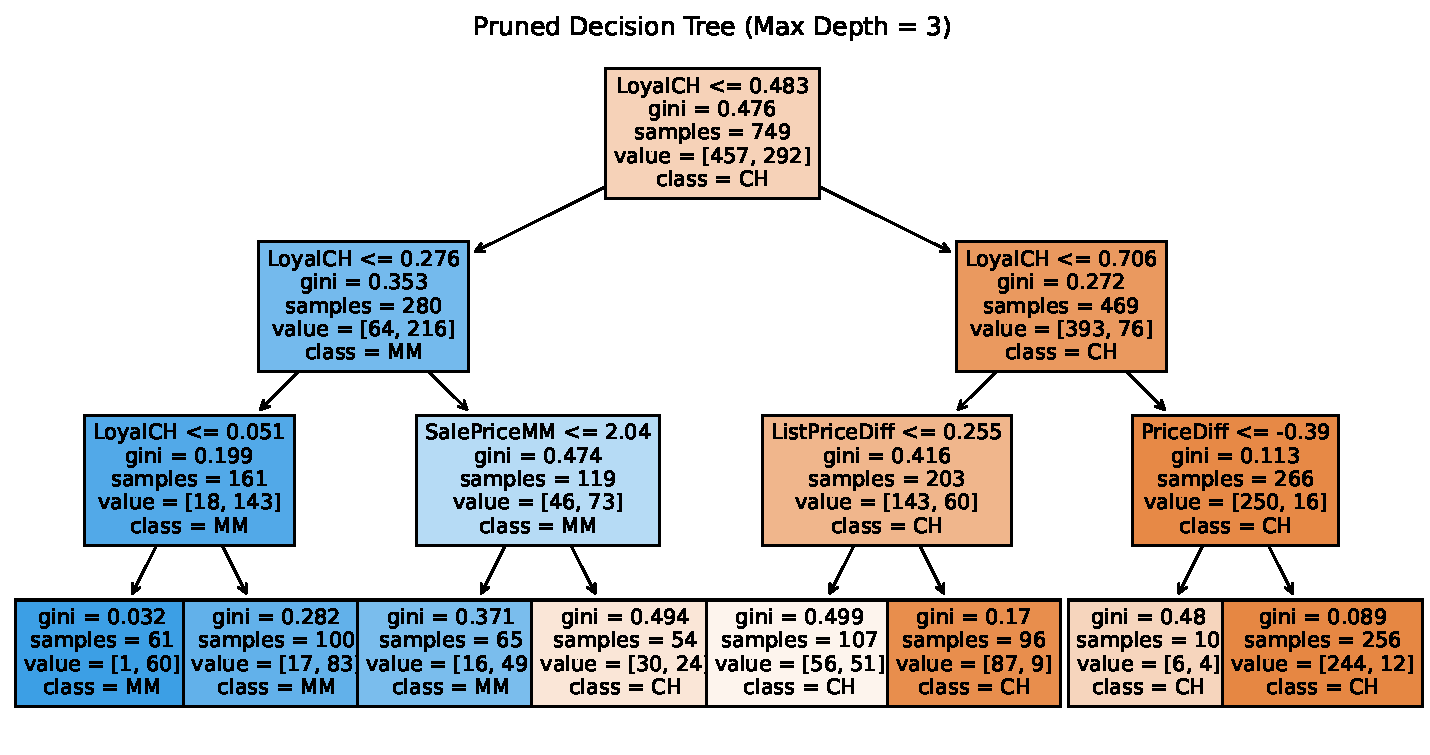
\includegraphics{PS4_files/figure-pdf/cell-13-output-2.pdf}

\begin{verbatim}
8
\end{verbatim}

\subsection{Question 3d}\label{question-3d}

\begin{Shaded}
\begin{Highlighting}[]
\CommentTok{\# predict on the test set and compute the confusion matrix}
\NormalTok{y\_test\_pred }\OperatorTok{=}\NormalTok{ tree\_clf.predict(X\_test\_encoded)}
\NormalTok{conf\_matrix }\OperatorTok{=}\NormalTok{ confusion\_matrix(y\_test\_encoded, y\_test\_pred)}

\CommentTok{\# display the test error rate}
\NormalTok{test\_error\_rate }\OperatorTok{=} \DecValTok{1} \OperatorTok{{-}}\NormalTok{ accuracy\_score(y\_test\_encoded, y\_test\_pred)}
\NormalTok{conf\_matrix, test\_error\_rate}
\end{Highlighting}
\end{Shaded}

\begin{verbatim}
(array([[160,  36],
        [ 41,  84]]),
 0.23987538940809972)
\end{verbatim}

\subsection{Question 3e}\label{question-3e}

\begin{Shaded}
\begin{Highlighting}[]
\CommentTok{\# perform CCP path to get alpha values}
\NormalTok{path }\OperatorTok{=}\NormalTok{ tree\_clf.cost\_complexity\_pruning\_path(X\_train\_encoded, y\_train\_encoded)}
\NormalTok{ccp\_alphas }\OperatorTok{=}\NormalTok{ path.ccp\_alphas[:}\OperatorTok{{-}}\DecValTok{1}\NormalTok{]}

\CommentTok{\# Perform 5{-}fold cross{-}validation}
\NormalTok{cv\_scores }\OperatorTok{=}\NormalTok{ []}

\ControlFlowTok{for}\NormalTok{ alpha }\KeywordTok{in}\NormalTok{ ccp\_alphas:}
\NormalTok{    pruned\_tree }\OperatorTok{=}\NormalTok{ DecisionTreeClassifier(ccp\_alpha}\OperatorTok{=}\NormalTok{alpha, random\_state}\OperatorTok{=}\DecValTok{2}\NormalTok{)}
\NormalTok{    scores }\OperatorTok{=}\NormalTok{ cross\_val\_score(pruned\_tree, X\_train\_encoded,}
\NormalTok{                             y\_train\_encoded, cv}\OperatorTok{=}\DecValTok{5}\NormalTok{, scoring}\OperatorTok{=}\StringTok{\textquotesingle{}accuracy\textquotesingle{}}\NormalTok{)}
\NormalTok{    cv\_scores.append(}\DecValTok{1} \OperatorTok{{-}}\NormalTok{ np.mean(scores))}

\CommentTok{\# find the optimal alpha}
\NormalTok{optimal\_alpha }\OperatorTok{=}\NormalTok{ ccp\_alphas[np.argmin(cv\_scores)]}

\CommentTok{\# display the plot}
\NormalTok{plt.figure(figsize}\OperatorTok{=}\NormalTok{(}\DecValTok{8}\NormalTok{, }\DecValTok{5}\NormalTok{))}
\NormalTok{plt.plot(ccp\_alphas, cv\_scores, marker}\OperatorTok{=}\StringTok{"o"}\NormalTok{, linestyle}\OperatorTok{=}\StringTok{"dashed"}\NormalTok{,}
\NormalTok{         label}\OperatorTok{=}\StringTok{"Cross{-}Validated Error Rate"}\NormalTok{)}
\NormalTok{plt.xlabel(}\StringTok{"Alpha (ccp\_alpha)"}\NormalTok{)}
\NormalTok{plt.ylabel(}\StringTok{"Classification Error Rate"}\NormalTok{)}
\NormalTok{plt.title(}\StringTok{"Cost Complexity Pruning: Alpha vs. Error Rate"}\NormalTok{)}
\NormalTok{plt.axvline(optimal\_alpha, color}\OperatorTok{=}\StringTok{"red"}\NormalTok{, linestyle}\OperatorTok{=}\StringTok{"dashed"}\NormalTok{,}
\NormalTok{            label}\OperatorTok{=}\SpecialStringTok{f"Optimal Alpha = }\SpecialCharTok{\{}\NormalTok{optimal\_alpha}\SpecialCharTok{:.4f\}}\SpecialStringTok{"}\NormalTok{)}
\NormalTok{plt.legend()}
\NormalTok{plt.show()}

\NormalTok{optimal\_alpha}
\end{Highlighting}
\end{Shaded}

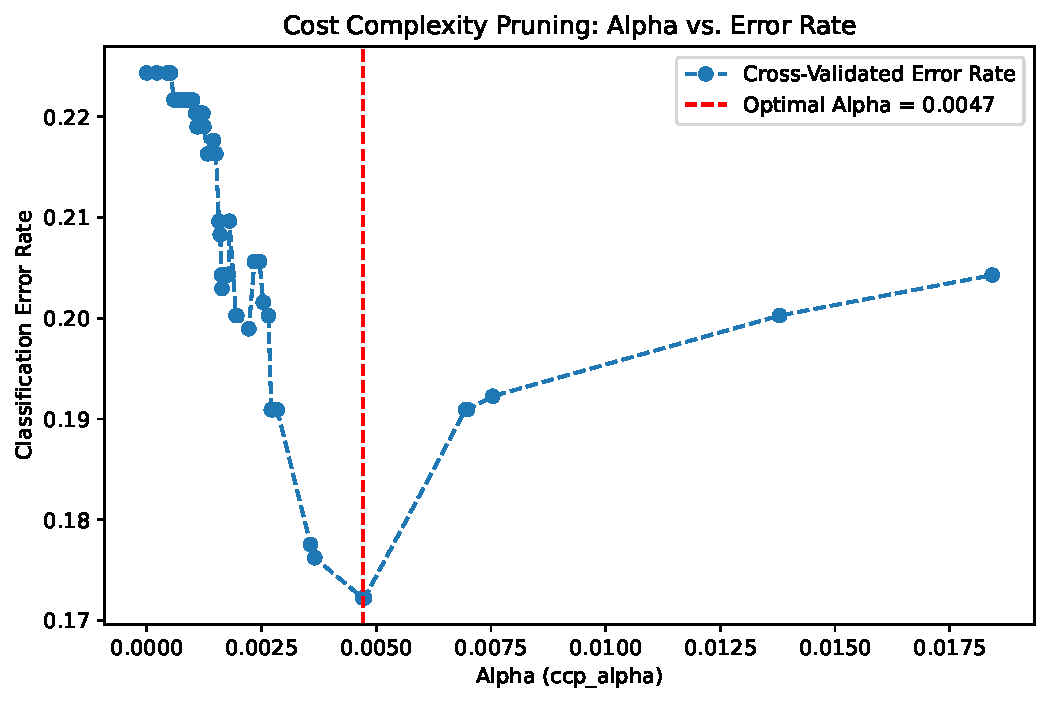
\includegraphics{PS4_files/figure-pdf/cell-15-output-1.pdf}

\begin{verbatim}
0.0047063975958152315
\end{verbatim}

\begin{itemize}
\tightlist
\item
  The optimal value of α corresponding to the lowest cross-validated
  classification error rate is 0.0047.
\end{itemize}

\subsection{Question 3f}\label{question-3f}

\begin{Shaded}
\begin{Highlighting}[]
\CommentTok{\# compute the tree size for each alpha}
\NormalTok{tree\_sizes }\OperatorTok{=}\NormalTok{ []}

\ControlFlowTok{for}\NormalTok{ alpha }\KeywordTok{in}\NormalTok{ ccp\_alphas:}
\NormalTok{    pruned\_tree }\OperatorTok{=}\NormalTok{ DecisionTreeClassifier(ccp\_alpha}\OperatorTok{=}\NormalTok{alpha, random\_state}\OperatorTok{=}\DecValTok{2}\NormalTok{)}
\NormalTok{    pruned\_tree.fit(X\_train\_encoded, y\_train\_encoded)}
\NormalTok{    tree\_sizes.append(pruned\_tree.tree\_.node\_count)}

\CommentTok{\# find the optimal tree size corresponding to the lowest classification error}
\NormalTok{optimal\_tree\_size }\OperatorTok{=}\NormalTok{ tree\_sizes[np.argmin(cv\_scores)]}

\CommentTok{\# display the plot}
\NormalTok{plt.figure(figsize}\OperatorTok{=}\NormalTok{(}\DecValTok{8}\NormalTok{, }\DecValTok{5}\NormalTok{))}
\NormalTok{plt.plot(tree\_sizes, cv\_scores, marker}\OperatorTok{=}\StringTok{"o"}\NormalTok{, linestyle}\OperatorTok{=}\StringTok{"dashed"}\NormalTok{,}
\NormalTok{         label}\OperatorTok{=}\StringTok{"Cross{-}Validated Error Rate"}\NormalTok{)}
\NormalTok{plt.xlabel(}\StringTok{"Tree Size (Number of Nodes)"}\NormalTok{)}
\NormalTok{plt.ylabel(}\StringTok{"Classification Error Rate"}\NormalTok{)}
\NormalTok{plt.title(}\StringTok{"Tree Size vs. Classification Error Rate"}\NormalTok{)}
\NormalTok{plt.axvline(optimal\_tree\_size, color}\OperatorTok{=}\StringTok{"red"}\NormalTok{, linestyle}\OperatorTok{=}\StringTok{"dashed"}\NormalTok{,}
\NormalTok{            label}\OperatorTok{=}\SpecialStringTok{f"Optimal Tree Size = }\SpecialCharTok{\{}\NormalTok{optimal\_tree\_size}\SpecialCharTok{\}}\SpecialStringTok{"}\NormalTok{)}
\NormalTok{plt.legend()}
\NormalTok{plt.show()}

\NormalTok{optimal\_tree\_size}
\end{Highlighting}
\end{Shaded}

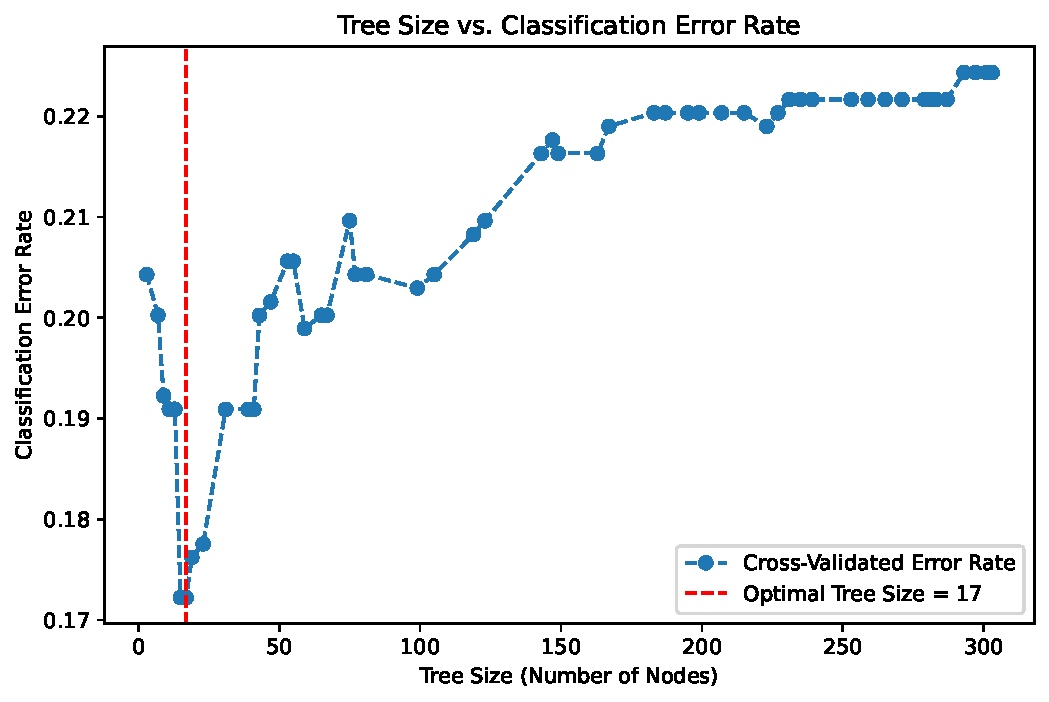
\includegraphics{PS4_files/figure-pdf/cell-16-output-1.pdf}

\begin{verbatim}
17
\end{verbatim}

\begin{itemize}
\tightlist
\item
  The optimal tree size corresponding to the lowest cross-validated
  classification error rate is 17 nodes.
\item
  The α (ccp\_alpha) parameter controls pruning by penalizing the
  complexity of the tree - higher values \hspace{0pt}\hspace{0pt}result
  in more aggressive pruning and smaller tree size. Smaller α allows for
  deeper trees, which reduces training error but can easily lead to
  overfitting and increase test error. Larger α simplifies the tree
  structure and improves generalization but can lead to underfitting.
  The ideal α value should balance model complexity and accuracy,
  preventing overfitting and underfitting, thereby minimizing
  classification error.
\end{itemize}

\subsection{Question 3g}\label{question-3g}

\begin{Shaded}
\begin{Highlighting}[]
\CommentTok{\# fit the pruned decision tree using the optimal alpha}
\NormalTok{optimal\_pruned\_tree }\OperatorTok{=}\NormalTok{ DecisionTreeClassifier(}
\NormalTok{    ccp\_alpha}\OperatorTok{=}\NormalTok{optimal\_alpha, random\_state}\OperatorTok{=}\DecValTok{2}\NormalTok{)}
\NormalTok{optimal\_pruned\_tree.fit(X\_train\_encoded, y\_train\_encoded)}

\CommentTok{\# display the pruned tree}
\NormalTok{plt.figure(figsize}\OperatorTok{=}\NormalTok{(}\DecValTok{12}\NormalTok{, }\DecValTok{6}\NormalTok{))}
\NormalTok{plot\_tree(optimal\_pruned\_tree, feature\_names}\OperatorTok{=}\NormalTok{X\_train\_encoded.columns,}
\NormalTok{          class\_names}\OperatorTok{=}\NormalTok{[}\StringTok{\textquotesingle{}CH\textquotesingle{}}\NormalTok{, }\StringTok{\textquotesingle{}MM\textquotesingle{}}\NormalTok{], filled}\OperatorTok{=}\VariableTok{True}\NormalTok{, fontsize}\OperatorTok{=}\DecValTok{10}\NormalTok{)}
\NormalTok{plt.title(}\SpecialStringTok{f"Optimal Pruned Decision Tree (ccp\_alpha = }\SpecialCharTok{\{}\NormalTok{optimal\_alpha}\SpecialCharTok{:.4f\}}\SpecialStringTok{)"}\NormalTok{)}
\NormalTok{plt.show()}
\end{Highlighting}
\end{Shaded}

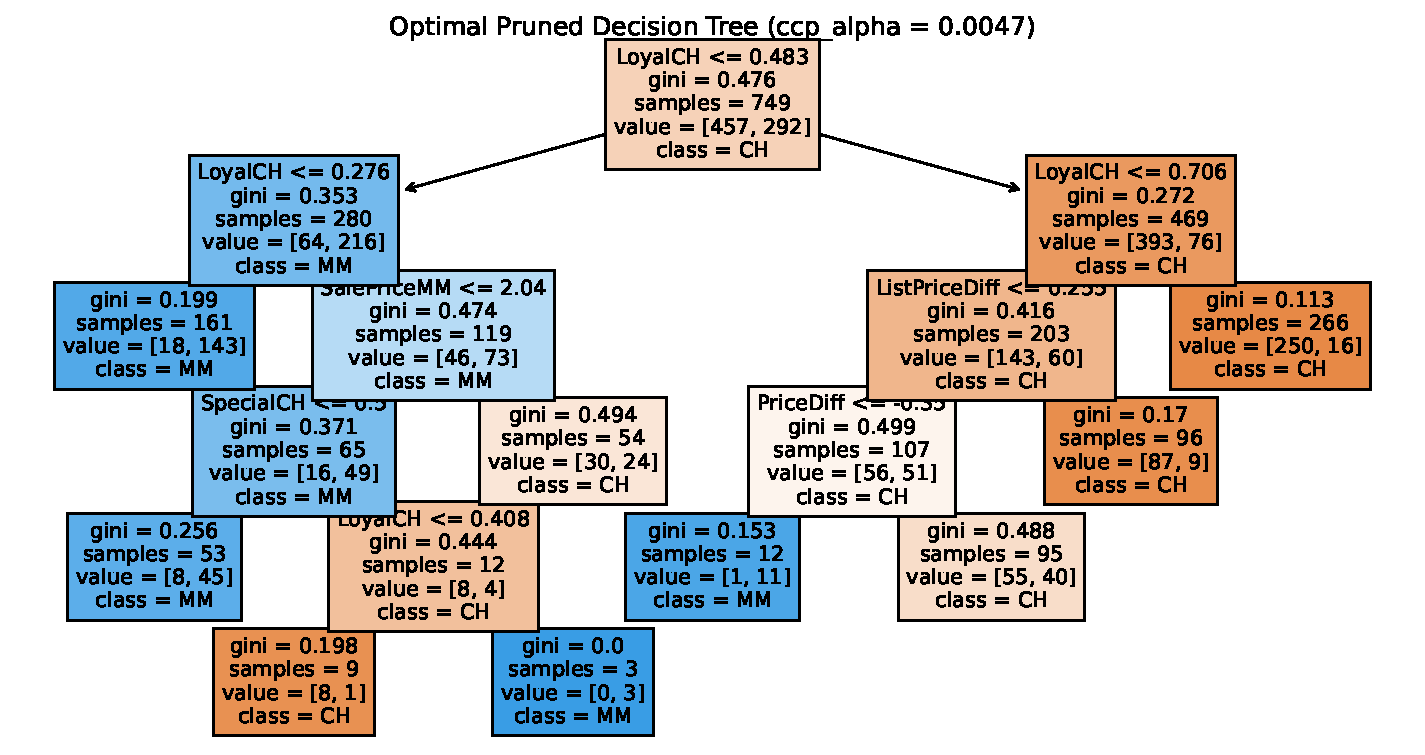
\includegraphics{PS4_files/figure-pdf/cell-17-output-1.pdf}

\subsection{Question 3h}\label{question-3h}

\begin{Shaded}
\begin{Highlighting}[]
\NormalTok{y\_train\_pred\_pruned }\OperatorTok{=}\NormalTok{ optimal\_pruned\_tree.predict(X\_train\_encoded)}
\NormalTok{train\_error\_rate\_pruned }\OperatorTok{=} \DecValTok{1} \OperatorTok{{-}} \OperatorTok{\textbackslash{}}
\NormalTok{    accuracy\_score(y\_train\_encoded, y\_train\_pred\_pruned)}

\CommentTok{\# compare training error rates}
\NormalTok{train\_error\_rate, train\_error\_rate\_pruned}
\end{Highlighting}
\end{Shaded}

\begin{verbatim}
(0.006675567423230944, 0.1562082777036048)
\end{verbatim}

\begin{itemize}
\tightlist
\item
  The training error rate for the unpruned tree is 0.67\%; the training
  error rate for the pruned tree is 15.62\%.
\item
  Pruning reduces the tree's complexity by removing branches that
  capture minor variations in the training data, making it less
  flexible. The unpruned tree overfits by memorizing the training data,
  resulting in an artificially low training error but a higher test
  error. \hspace{0pt}\hspace{0pt}
\end{itemize}

\subsection{Question 3i}\label{question-3i}

\begin{Shaded}
\begin{Highlighting}[]
\NormalTok{y\_test\_pred\_pruned }\OperatorTok{=}\NormalTok{ optimal\_pruned\_tree.predict(X\_test\_encoded)}
\NormalTok{test\_error\_rate\_pruned }\OperatorTok{=} \DecValTok{1} \OperatorTok{{-}}\NormalTok{ accuracy\_score(y\_test\_encoded, y\_test\_pred\_pruned)}

\CommentTok{\# compare test error rates}
\NormalTok{test\_error\_rate, test\_error\_rate\_pruned}
\end{Highlighting}
\end{Shaded}

\begin{verbatim}
(0.23987538940809972, 0.19626168224299068)
\end{verbatim}

\begin{itemize}
\tightlist
\item
  The test error rate for the unpruned tree is 24.3\%; the test error
  rate for the pruned tree is 19.63\%. -Pruning removes overly specific
  splits that capture noise in the training data, preventing
  overfitting. As a result, the pruned tree generalizes unseen data
  better, reducing test errors. The unpruned tree overfits the training
  set, leading to a higher test error due to poor generalization.
\end{itemize}




\end{document}
